\section{Geschichtliche Entwicklung}
\label{ch:history}

Um die Notwendigkeit der serviceorientierten Architektur nachvollziehen zu können, lohnt es sich die Vergangenheit - vor SOA - anzusehen. In diesem Kapitel wird die Entwicklung von Software-Architekturen vom Monolithen bis hin zur Serviceorientiertheit betrachtet.

\subsection{Monolithische Architektur}
\label{sec:monolithicArch}

Als monolithisch werden Objekte bezeichnet, die \glqq aus einem Stück bestehen[.]; zusammenhängend und fugenlos [sind]\grqq{} \cite{Duden.monolithisch.25.10.2022}. Im Kontext des Software-Engineerings sind damit jegliche Anwendungen gemeint, deren Module nicht unabhängig voneinander ausgeführt werden können und deren Funktionalitäten in einer Applikation gekapselt sind \cite{Ponce.2019}.

Während den Anfängen des Software-Engineerings und bevor das Fachgebiet der Software-Architektur existiert hatte, existierten fast ausschließlich Monolithen \cite{Kruchten.2006}.  

Ende der 1960er Jahre gab es die ersten Bemerkungen, Software nicht nur als \glqq amorphous lump of program\grqq{} \cite{Kruchten.2006}[S.24] anzusehen, sondern gezielt die Architektur eines Software-Systems zu designen.

Monolithen haben noch heute ihre Daseinsberechtigung. Gerade kleine stand-alone Anwendungen werden häufig von einem Service dargestellt. Der große Vorteil dabei ist das einfache Testen \cite{Ponce.2019}. Einzelne Dienste einer Anwendung müssen nicht mit Integrationstests auf verschiedenen Status abgebildet werden, da es nur einen Dienst zum Testen gibt. Auch das Deployment ist simpel, da es nur aus einer ausführbaren Komponente besteht. 

Durch die \glqq fehlende\grqq{} Architektur wird zunächst Zeit gewonnen, da weniger geplant werden muss. Für kleine Projekte oder Prototypen ist das ideal. Gerade bei Letzterem können durch den erstmaligen Aufbau im Monolith die Komplexität und einzelne Komponenten erforscht werden \cite{Ponce.2019}. Aber bei großen Projekten geht schnell der Überblick verloren und die Entwicklung kommt ins Stocken \cite{Ponce.2019}. 

Die Entwicklung einer monolithischen Anwendung bedeutet eine enge Bindung zur genutzten Technologie \cite{Ponce.2019}. Falls der Support verwendeter Drittanbieter-Software ausläuft, oder neue Schwachstellen gefunden werden, ist es nur schwer möglich Änderungen vorzunehmen. Und gleichzeitig: Egal wie groß oder klein eine Anpassung ist, die gesamte Anwendung muss immer neu getestet, gebaut und verteilt werden. Falls ein Laufzeitfehler auftritt, hat dies den Absturz der gesamten Anwendung zur Folge \cite{Ponce.2019}. Und obwohl solch ein Bug durch eine kleine Modifikation gefixt werden kann. Manchmal ist ein neuer Build zu aufwändig und es wird auf mehrere Änderungen gewartet. Darunter leidet die Qualität der Software. Auch lässt sich die Applikation nicht beliebig skalieren. Durch zum Beispiel Load Balancer kann die gesamte Anwendung horizontal skalieren, nicht jedoch einzelne Komponenten.

Zusammenfassend: Monolithen sind gut für kleine Projekte, oder erste Proof of Concepts. Falls eine Software jedoch nachhaltig, mehrere Jahre lang zuverlässig betreut und weiterentwickelt werden soll, steigt die Komplexität dieser drastisch mit der Zeit. Neue Teammitglieder müssen sich teilweise in die komplette Codebase einarbeiten, um Änderungen vorzunehmen. Es kann auch dazu kommen, dass keine neuen Arbeitskräfte gefunden werden die sich mit 20 Jahre alter Software-Technologie auseinandersetzen wollen und somit ist eine Neuentwicklung früher oder später unumgehbar. 

Wenn Architekturen - und damit der Aufbau von Software - verglichen werden, dann wird dies mithilfe von \glqq fundamentalen Grundprinzipien\grqq{} getan \cite{FrankBuschmann.}. Im Folgenden werden diese Punkte aufgezählt um zu zeigen, gegen welche Grundprinzipien die monolithische Architektur verstößt. In den darauf folgenden Kapiteln werden Architekturen gezeigt die iterativ verschiedene Probleme lösen, welche letztendlich einen historischen Verlauf zu SOA aufzeigen soll:
\begin{itemize}
    \item \textbf{Abstraktion}: \glqq Die essenziellen Eigenschaften eines Objekts, die es von allen anderen Arten von Objekten unterscheidet und somit klar definierte konzeptionelle Grenzen in Bezug auf die Perspektive des Betrachters setzt\grqq{} \cite{Booch.1993}. In einem Monolith kann es keine echte Abstraktion geben, da die Software nur aus einem Objekt - sich selbst - besteht. Natürlich existieren auf einem niedrigeren Level eine Abstraktion, aber nicht in der Architektur selbst.
    \item \textbf{Kapselung}: Durch die Verkapselung verschiedenster Abstraktionen können diese gruppiert und auseinander gehalten werden. Dies fördert die Änderbarkeit und Wiederverwendbarkeit \cite{FrankBuschmann.}. Die Kapselung, zum Beispiel von Klassen einer Programmiersprache kann auch für Monolithen existieren, aber nicht in einer Form, die eine Wiederverwendbarkeit anstrebt.
    \item \textbf{Modularisierung}: Hierbei geht es um die sinnvolle Zerlegung eines Softwaresystems und dessen Gruppierung in Subsysteme und Komponenten. Module dienen als physische Container für Funktionalitäten oder Verantwortlichkeiten einer Anwendung. \cite{FrankBuschmann.}. Wie bei vielen dieser Prinzipien lässt die monolithische Architektur Modularisierung zu einem gewissen Grad zu, aber nur auf einem niedrigen Level.
    \item \textbf{Trennung von Verantwortlichkeiten}: Unterschiedliche Verantwortlichkeiten innerhalb eines Softwaresystems sollten voneinander getrennt werden. 
    \item \textbf{Kopplung und Kohäsion}: Die Kopplung ist das Maß für die Stärke der Assoziation zwischen Modulen. Eine Starke Kopplung verkompliziert das System \cite{FrankBuschmann.}. Kohäsion misst den Grad der Konnektivität zwischen den Funktionen und Elementen eines einzelnen Moduls.
    \item \textbf{Suffizienz, Vollständigkeit und Primitivität}: Suffizienz meint, dass eine Komponente alle notwendigen Merkmale einer Abstraktion erfasst und eine sinnvolle und effiziente Interaktion ermöglicht. Vollständigkeit heißt, dass alle relevanten Merkmale erfasst werden. Mit Primitivität ist gemeint, dass jede Operation, die eine Komponente ausführen kann, einfach implementiert werden kann \cite{FrankBuschmann.}.
    \item \textbf{Single Point of Reference}: Jede Entität innerhalb eines Softwaresystems sollte nur einmal definiert werden. Dadurch entstehen keine inkonsistenten Zustände.
\end{itemize}

\subsection{Schichtenarchitektur}
\label{sec:layeredArch}

Die Schichtenarchitektur war eines der ersten Architektur-Pattern mit welchem versucht wurde die Probleme einer monolithischen Architektur zu lösen \cite{SavolainenJuha.2009} und ist bis heute wahrscheinlich einer der am häufigsten angewendeten Software-Architekturen (vor allem im Web).

Ein Programm wird dabei in $n$ Schichten aufgeteilt, jede Schicht ist ein Modul der Software und kommuniziert über Protokolle mit anderen Schichten. Die Aufteilung alleine löst schon fast alle oben genannten Probleme. Die Schichten bilden meist eine Hierarchie ab, wobei die Kommunikation nur strikt durch gewisse Schichten geschieht. 

Vor allem lassen sich Verantwortlichkeiten sehr gut damit trennen. Als Beispiel, kann das 3-Schichten Modell aus typischen Web-Anwendungen betrachtet werden\footnote{Auch wenn dies ein prominentes Beispiel ist, besteht eine Schichtenarchitektur nicht immer aus 3 Schichten}:
\begin{enumerate}
    \item \textbf{Präsentationsschicht}: das Frontend als grafische Benutzeroberfläche im Browser.
    \item \textbf{Anwendungsschicht}: die eigentliche Funktionalität der Software abgeschottet von Anwendenden.
    \item \textbf{Datenschicht}: eine Datenbank, auf der die Anwendungsdaten verwaltet werden.
\end{enumerate}

Bei der Modellierung können die Schichten einzeln betrachtet werden, um Schnittstellen zu definieren. Entwicklerteams können daraufhin gleichzeitig an Front- und Backend arbeiten und sind dabei technologisch unabhängig voneinander. Und im Laufe des Lebenszyklus der Anwendung können einzelne Schichten ausgetauscht werden, um neue Technologie einzusetzen. Weitere Vorteile sind auch, dass sich die Geschäftslogik direkt im Code befindet und dass geheime Informationen nicht öffentlich für Benutzer zugänglich sind, sondern sich auf einer unzugänglichen Schicht befinden.

Für große Projekte mit größeren Teams ist es leichter Software in Schichten zu schreiben. Einzelne Teams können sich dabei auf eine bestimmte Schicht spezialisieren, um effizienter zu sein. 

Die Verteilung von Software bringt auch Nachteile mit sich, bzw. alle Vorteile der monolithischen sind die Nachteile von dieser Architektur:
\begin{itemize}
    \item Das Testen ist wesentlich aufwändiger. Unit-Tests sind auf den einzelnen Schichten unverändert, aber bei der Integration aller Schichten ist es schwer alle Testfälle abzudecken bzw. die Tests überhaupt zu schreiben.
    \item Die Installation von Software ist wesentlich aufwändiger, da mehrere Schichten meist über das Internet kommunizieren müssen.
    \item Der Planungsaufwand ist höher und vor allem kleine Projekte könnten unnötig Zeit an der Trennung der Schichten verlieren. Macht sich aber in der späteren Betreuung des Codes bezahlt.
\end{itemize}

Zusammengefasst lässt sich sagen: Die Schichtenarchitektur teilt \textbf{eine} Software in \textbf{verschiedene} Schichten auf. Dabei muss stets auf die Balance zwischen Kopplung und Kohäsion geachtet werden. Die Schichten können dabei verschiedenste Technologien implementieren, solange diese mithilfe wohl definierter Protokolle kommunizieren können. Die Schichten können in der Entwicklung anderer Software wiederverwendet werden, was die Entwicklung in Zukunft erleichtert. Aber die Architektur zeigt ebenfalls Probleme auf. Die Schichten trennen zwar zu einem gewissen Grad die Verantwortlichkeiten der Software, aber für große Projekte ist die statische Hierarchie der Schichten nicht fördernd. Oftmals werden bei einer 3-Schichten Architektur auch nur 2 große Monolithen entwickelt (mit einer Datenschicht) \cite{FrankBuschmann.}. 

\subsection{Serviceorientierte Architektur}
\label{sec:historySoa}

Die Herausforderung der Schichtenarchitektur kann gelöst werden, indem die \glqq Schichten\grqq{} granularer werden. Und anstatt diese in einer festen Hierarchie anzuordnen - wo zum Beispiel Schicht $n$ nur mit Schicht $n+1$ kommuniziert - gibt es eine liberalere Kommunikation, die nicht mehr statisch vorgegeben sein muss. Anstatt, dass eine Schicht für die gesamte Geschäftslogik einer Anwendung zuständig ist, werden weitere Verantwortlichkeiten innerhalb dieser in Services aufgeteilt. Dadurch wird eine losere Kopplung und eine erhöhte Kohäsion erreicht. 

Dieses Ziel hat gerade für große Softwareunternehmen einen immensen Vorteil. Anstatt einzelne Services nur in der Entwicklung wiederzuverwenden, können diese jetzt zur Laufzeit wiederverwendet werden. Die Verantwortlichkeiten sind so granular, dass sich diese in anderen Projekten unverändert wiederverwenden kann.

Langfristig bilden sich nur geringe Kosten durch den hohen Grad der Wiederverwendbarkeit der Dienste, aber bei diesem Grad der Granularität stößt die serviceorientierte Architektur an einen großen Overhead der auch Probleme mit sich bringt \cite{SolutionsMartinSchmidtAsgard.26.11.2022}:\begin{itemize}
    \item Die Analyse, Konzeption und Implementierung ist initial wesentlich höher als bei anderen Architekturen.
    \item Die Wiederverwendbarkeit kann auch ein Problem darstellen, da dies nur eingeschränkt und nur auf sehr langer Zeit gesehen möglich ist. Das erfordert eine noch genauere Planung für die Zukunft.
    \item Die Granularität erhöht die Anzahl der Schnittstellen, deren Änderungen oftmals zu Kompatibilitätsproblemen führen können (=erhöhte Komplexität).
    \item In der Regeln hat eine SOA-Anwendung eine schlechtere Performance und höheres Datenvolumen, da die Dienstkommunikation höhere Latenzen darstellt.
    \item Die Bereitstellung und Konfiguration der Bindung zwischen den Diensten ist häufig komplex und Themen wie die Authentifizierung/Autorisierung sind Herausforderungen die mit hohen Kosten verbunden sind.
    \item Entwicklerteams müssen über ein breiteres Wissen verfügen um SOA wirklich anwenden zu können.
    \item Die Kostenverwaltung der Entwicklung einer zentralen und Abteilungsübergreifenden SOA ist eine politische Herausforderung und muss von Mitarbeitenden unterstützt werden.
\end{itemize}

Die Information, die aus diesem Kapitel herausstechen sollte, ist die Tatsache, dass sich SOA erst bezahlbar macht, nachdem die gesamte Architektur steht. Bis zu diesem Punkt sind immense Aufwände seitens des Unternehmens notwendig. Bei kleinen bzw. neuen Softwareunternehmen ist der Systemaufbau mit SOA meist zu teuer und würde sich nicht lohnen, bzw. bei einer Gründung ist es schwer in die Zukunft zu blicken, um die richtigen Services herauszusuchen. Für bestehende Unternehmen heißt eine SOA, die Neuentwicklung der Softwarelandschaft. Ein Transformationsprojekt hin zu SOA kann Jahre dauern und ist ein großes  für die Zukunft. Die abgeschlossene Transformation macht sich jedoch bezahlt. 

Interessant zu sehen: bei diesen Architekturen gibt es einen Trade-off zwischen Komplexität in der Planung und der Komplexität in der Pflege/Entwicklung. Die Gesamtkosten eines Projektes sollten unabhängig von der Wahl einer Architektur sein, jedoch werden die Kosten und Aufwände anders über den Projektlebenszyklus verteilt. 

\newpage
Monolithen haben wenig initiale Aufwände, aber die spätere Pflege ist mit einem hohen Kostenaufwand verbunden. SOA hat immense Anfangskosten, welche nach dem Aufbau der Architektur wieder fallen. Und die Schichtenarchitektur ist eine Balance dazwischen. Monolithische Projekte können ohne viel Aufwand angefangen werden und falls diese ohne Abschluss scheitern, so wurde nur der minimale Aufwand erreicht. Im Gegensatz dazu kostet ein gescheitertes SOA-Projekt wesentlich mehr Geld und Aufwände, da das meiste davon in der Planung (am Anfang) aufgebracht wird.

\begin{figure}[H]
    \centering
    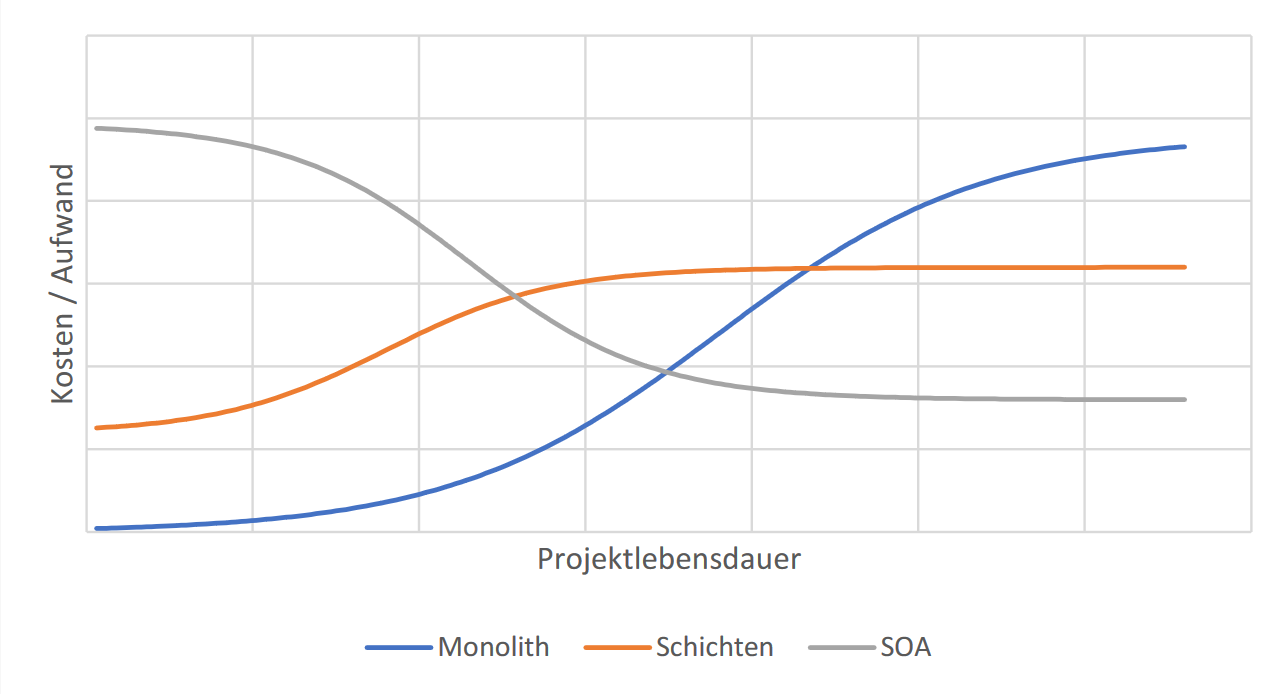
\includegraphics[width=.9\textwidth]{images/archgraph.png}
    \caption{Relativer Kosten-/Aufwand-Vergleich der vorgestellten Architekturen}
\end{figure}

Trotzdem kann sich der Umstieg zu einer serviceorientierten Architektur lohnen. Im Nachfolgendem wird tiefer darauf eingegangen wie sich SOA auf den Entwicklungs- und Auslieferungsprozess in der agilen Softwareentwicklung auswirkt.
